\newpage
\section{Дерево операций}
\label{sec:optree}

\subsection{Актуальность применения подхода SSA}

Как уже было упомянуто, один из этапов компиляции -- синтаксический анализ.
Реализующий модуль, получая на вход список токенов, в качестве выхода строит синтаксическое дерево.
Такое дерево, помимо прочего, обладает определенными особенностями, среди которых были выделены преимущества и недостатки.

Преимущества:

\begin{itemize}
    \item Синтаксическое дерево легко строится напрямую из списка токенов (или даже текста программы, если лексический анализ совместить с построением дерева) за один проход фактически без дополнительных структур данных.
    \item Синтаксическое дерево является представлением входной программы один-в-один (текст программы может быть восстановлен путем полного обхода дерева), поэтому удобно предоставлять диагностику пользователю (указание точного места в исходном коде).
\end{itemize}

Недостатки:

\begin{itemize}
    \item Процесс семантического анализа дерева нетривиален. Требуется задействовать дополнительные структуры данных для упорядочения информации (список переменных, функций) и т. д.
    \item Применение существенных трансформаций (оптимизаций) является трудоемким: для обнаружения и проверки инвариантов требуется выполнять обходы по несколько раз (анализ использования переменных, вывод типов, поиск определений), что верно и для замены узлов дерева.
\end{itemize}

Для разрешения описанных трудностей, связанных, в частности, с анализом потока данных для выполнения трансформаций, было предложено использовать подход, похожий на SSA.

SSA (static single assignment, статическое единственное присвоение) -- это представление программы, в котором у каждой переменной есть единственное определение, сопровождающееся инициализацией. Следующие примеры псевдокода демонстрируют одну и ту же программу, записанную в произвольной форме и в форме SSA.

\begin{lstlisting}[language=C++, caption=Программа в произвольной форме]
x = 1
y = x + 1
x = 2
z = x + 1
\end{lstlisting}

\begin{lstlisting}[language=C++, caption=Программа в форме SSA]
x1 = 1
y = x1 + 1
x2 = 2
z = x2 + 1
\end{lstlisting}

Используя свойство единственности присваивания, можно отследить, как было получено то или иное значение, обойдя цепочку определений и использований переменных.

В классическом подходе SSA, используемом в современных компиляторах, все высокоуровневые конструкции языка, такие как ветвления и циклы, разбиваются на последовательность базовых блоков программы, между которыми явно указываются переходы.
Кроме того, вводится понятие \(\phi\)-узлов, связывающих пути, по которым приходит определение переменной из разных блоков при нелинейном исполнении.

В настоящей работе была реализована структура данных, использующая подход SSA в упрощенной форме, достаточной для достижения поставленных целей.
Эта структура, названная деревом операций, описана далее.

\subsection{Описание дерева операций}

Дерево операций -- это дополнительное промежуточное представление исходной программы.
В общем случае узлами дерева являются операции, которые обмениваются между собой значениями, каждое из которых определяется своим типом.

Как видно на рисунке~\ref{fig:optree_scheme}, операция может иметь произвольное число операндов, не более одного результата, произвольное число атрибутов (вспомогательных данных, независимых от других операций), произвольное число вложенных операций внутри, а также объемлющую операцию, в теле которой указанная операция и находится.

\begin{figure}[h]
    \centering
    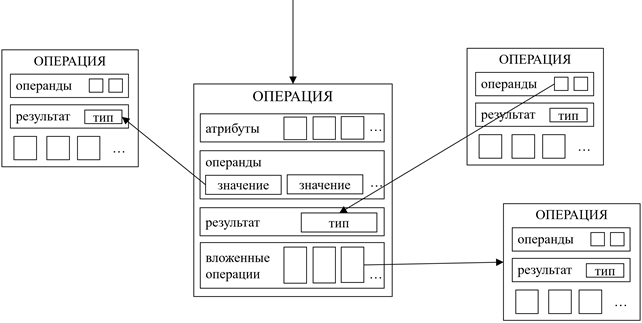
\includegraphics[width=\textwidth]{images/optree-scheme.png}
    \caption{Дерево операций.}
    \label{fig:optree_scheme}
\end{figure}

\textbf{Операция} владеет внешними значениями (результатами) и внутренними регистрами.
Результаты видны соседям операции и могут быть операндами других операций, но не видны операциям внутри тела.
Внутренние регистры, наоборот, доступны для использования операциями внутри тела, но снаружи не видны (как переменные во вложенном блоке в C++).
Операция не владеет операндами, так как это результаты или внутренние регистры других операций.
Также внутри хранится имя операции и код, определяющий ее вид (см. п.~\ref{sec:optree_rtti}).

\textbf{Значение} -- это единоразово определяемый неизменяемый регистр (как const переменная в C++).
Значение нельзя <<изменить>>, но можно создать новую операцию, которая будет иметь нужное значение в качестве результата, а старое значение отбросить (при необходимости удалить порождающую его операцию из дерева).
Значение хранит внутри себя породившую операцию, тип, список использований (операций, среди операндов которых есть указанное значение).

\textbf{Тип} -- это характеристика представления значения; неизменяемая структура, содержащая информацию, полезную для, собственно, представляемого типа.
Система типов в дереве операций сходна с системой типов компилируемого языка.

\textbf{Атрибут} -- это вспомогательные данные, которые используются для анализа операции (какое-либо численное значение, тип, подвид операции, строка и так далее).
Например, операция, описывающая функцию, может иметь имя функции и тип в качестве атрибутов, а операция, описывающая объявление константы - значение и тип константы и т. д.

К особенностям дерева операций можно отнести следующее:

\begin{itemize}
    \item Дерево операций можно построить из синтаксического дерева за один проход.
    \item Анализ использования значения представляет собой обход готового списка.
    \item Добавление или изменение операций прозрачно: операция хранит информацию о своем положении в дереве, значение хранит информацию о связанной операции и типе.
    \item Невозможно восстановить текст исходной программы напрямую, но можно ссылаться на исходный код в диагностике для пользователя, если сохранить ссылки на места в коде внутри операций при их создании из улов синтаксического дерева.
\end{itemize}

Для перевода синтаксического дерева в дерево операций был разработан модуль «конвертер».
Принцип работы конвертера, то есть, построения дерева операций состоит в обходе синтаксического дерева и создании операций в соответствии с типом и структурой узла синтаксического дерева с помощью вспомогательной инфраструктуры для вставки узлов.

\subsection{Динамическая идентификация типов операций}
\label{sec:optree_rtti}

Динамическая идентификация типа данных (run-time type identification, RTTI) -- механизм в некоторых языках программирования, который позволяет определить тип данных переменной или объекта во время выполнения программы.
Существует множество реализаций такого механизма, но наиболее распространёнными являются:

\begin{itemize}
    \item таблица указателей на объекты;
    \item хранение информации об объекте в памяти вместе с ним.
\end{itemize}

Таким образом, операция определения типа сводится либо к поиску в таблице, либо к просмотру нескольких байт до адреса, на который указывает указатель на объект.
У каждого способа есть свои преимущества и недостатки.
К примеру, в первом случае для определения типа переменной, требуются некоторые операции поиска по таблице указателей.
А во втором случае, переменные начинают занимать больше места в оперативной памяти, чем ожидается, ведь к их известному размеру добавляется некоторое количество байтов, нужных для идентификации их типа.

В настоящей работе для операций используется второй подход.
Для создания операций конкретного типа используются классы-адаптеры, каждый из которых представляет определенную операцию и имеет, помимо прочего, статический метод, возвращающий идентификтор типа операции.

\begin{lstlisting}[language=C++, caption=Фрагмент реализации RTTI]
struct ConcreteOp : public BaseOp {
    // …

    static Operation::SpecId getSpecId() {
        static char specId = 0;
        return &specId;
    }

    static bool implementsSpecById(Operation::SpecId specId) {
        return specId == getSpecId() || BaseOp::implementsSpecById(specId);
    }
};
\end{lstlisting}

Таким образом, при создании конкретной операции в нее также записывается значение идентификтора типа операции из связанного адаптера. Это позволяет реализовать для класса операции следующие методы, использующие RTTI:

\begin{lstlisting}[language=C++, caption=Интерфейс для доступа к RTTI]
struct Operation {
    using SpecId = void *;
    SpecId specId;
    // …

public:
    template <typename AdaptorType> bool is() const;
    template <typename AdaptorType> AdaptorType as();
    template <typename AdaptorType> AdaptorType findParent() const;
    // …
};
\end{lstlisting}

Эти методы позволяют проверить, является ли операция конкретной операцией, привести ее к указанному типу, а также найти в дереве операций среди предков узла операцию, имеющую определенный тип. Реализованный механизм применяется во многих компонентах проекта, работающих с деревом операций, например, в семантическом анализаторе.

\subsection{Обзор поддерживаемых операций}

TODO
